\lecture{Infinte factorisaion of multiple non-parametric views}{multiview}

\begin{frame}
	\frametitle{Introduction}
	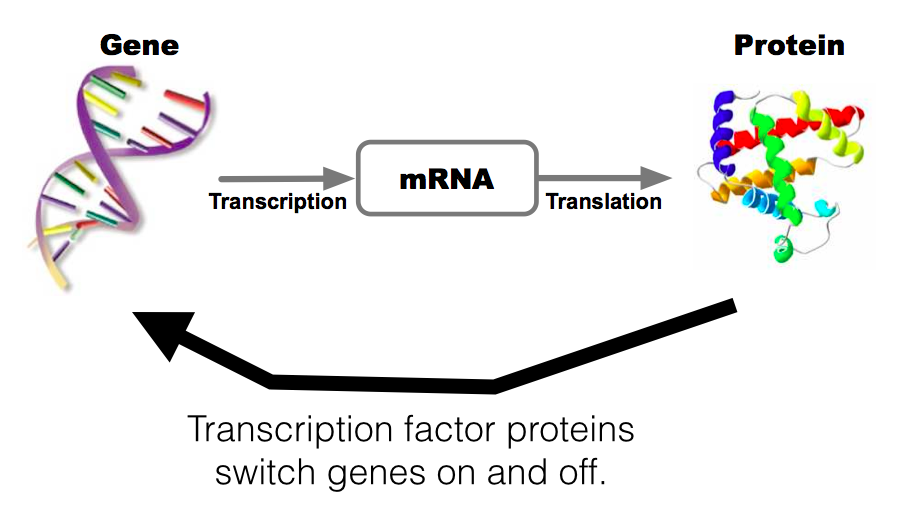
\includegraphics[width=\linewidth]{dogma}
	\begin{itemize}
		\item How related are mRNA and protein?
		\item {\bf Where is the external control?}
	\end{itemize}
\end{frame}

\begin{frame}
	\frametitle{Data}
	\begin{itemize}
		\item mRNA and protein time series for $\sim 500$ genes
	\end{itemize}
	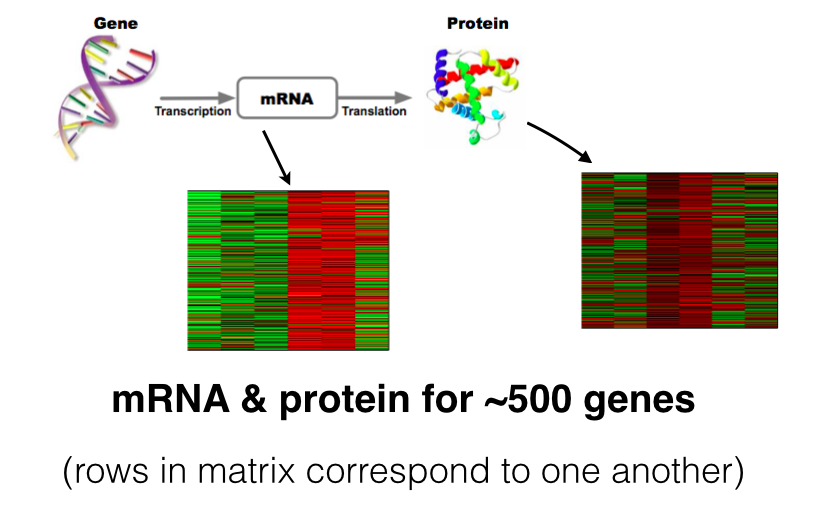
\includegraphics[width=\linewidth]{multiview_data}
\end{frame}

\begin{frame}
	\frametitle{Most don't look correlated}
	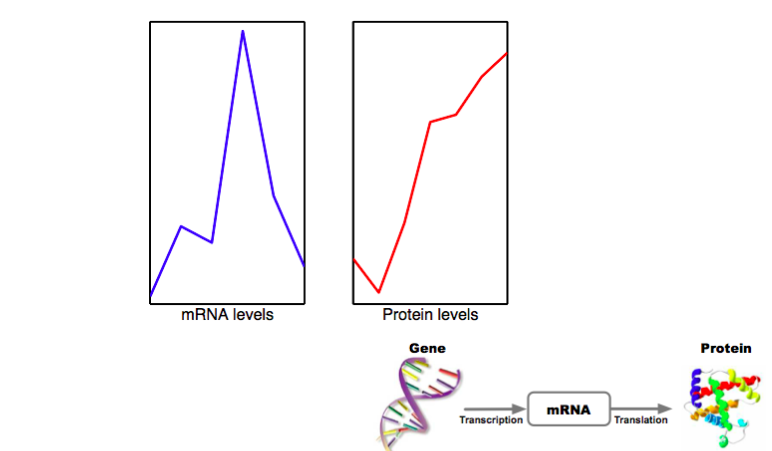
\includegraphics[width=\linewidth]{correlation}
	\begin{itemize}
		\item Most don't look correlated.
		\begin{itemize}
			\item Time delays? Saturation? Decay rates? Post-transcriptional control?
		\end{itemize}
	\end{itemize}
\end{frame}

\begin{frame}
	\frametitle{\emph{Non-parametric} relationships}
	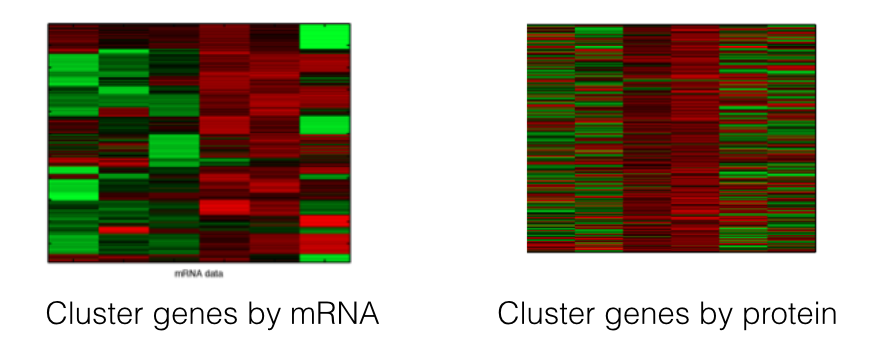
\includegraphics[width=\linewidth]{cluster_genes}
	\begin{itemize}
		\item Use clustering to define similarity.
		\item If genes A,B,C and D cluster together on both sides, then profiles are similar
		\begin{itemize}
			\item They are controlled by similar processes
		\end{itemize}
	\end{itemize}
\end{frame}

\begin{frame}
	\frametitle{Generative coupled mixture model}
	\begin{itemize}
		\item In \href{http://dx.doi.org/10.1093/bioinformatics/btn553}{Rogers et.~al 2008} we developed a generative linked cluster model
		\item Prior membership of gene $n$ in proteomic cluster $j$ was dependent on assignment of mRNA to cluster $k$:
		\[
		P(z_{nj}=1,z_{nk}=1) = P(z_{nj}=1|z_{nk}=1)P(z_{nk}=1)
		\]
		\item<2->Note that another obvious way to factorise this joint it to assume independence:
		\[
		P(z_{nj}=1,z_{nk}=1) = P(z_{nj}=1)P(z_{nk}=1)
		\]
		\item<2->I.e. cluster them separately
		\item<3->When we do inference, we can find the links between clusters
	\end{itemize}
	
\end{frame}

\begin{frame}
	\frametitle{Lots of links}
	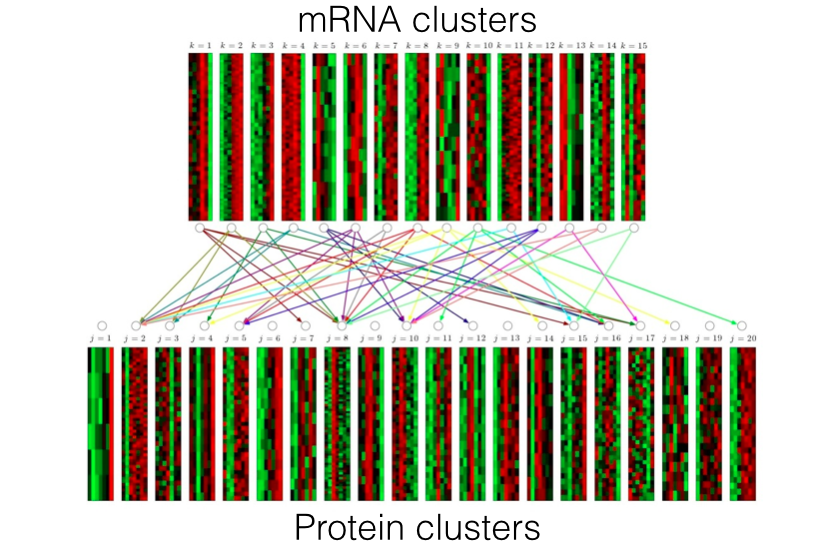
\includegraphics[width=\linewidth]{mesh}
	\begin{itemize}
		\item If all control before transcription, we would expect sparse links.
		\item That doesn't happen!
	\end{itemize}
\end{frame}

\begin{frame}
	\frametitle{Ribosomes}
		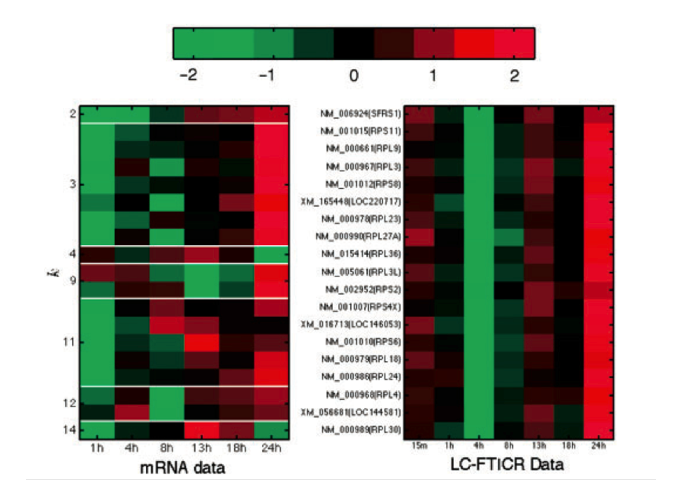
\includegraphics[width=0.8\linewidth]{ribosomes}
		\begin{itemize}
			\item Some strong links
			\item These are all ribosomal proteins
			\item The ribosome is where proteins are constructed
			\item Makes sense for them to be tightly transcriptionally controlled
		\end{itemize}
\end{frame}

\begin{frame}
	\frametitle{Crazy genes}
	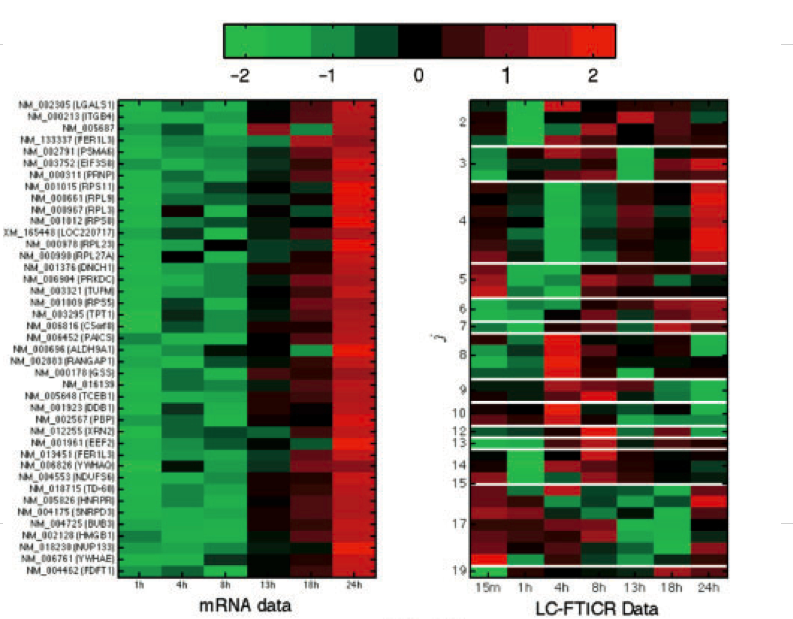
\includegraphics[width=0.8\linewidth]{chaos}
	\begin{itemize}
		\item In some cases, profiles were all over the place
		\item Here, highly conserved mRNA profiles, diverse protein profiles
	\end{itemize}
\end{frame}

\begin{frame}
	\frametitle{More flexible models}
	\begin{itemize}
		\item At this point, we thought about more flexible models (!)
		\item In particular, how about decomposing the joint density as:
		\[
			P(z_{nk}=1,z_{nj}=1) = \sum_i P(z_{nk}=1|i)P(z_{nj}=1|i)P(i)
		\]
		\item Each latent factor ($i$) defines a distribution over mRNA and protein clusters
		\item Use DP priors on $i$ and the clusters in the two \emph{views}
	\end{itemize}
\end{frame}

\begin{frame}
	\frametitle{Contingency tables}
	\begin{multicols}{2}
		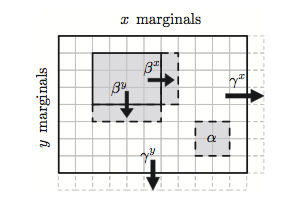
\includegraphics[width=\linewidth]{contingency}
	\newpage
	\begin{itemize}
		\item Can visualise $P(j,k)$ as a table
		\item Each $i$ is a block (if the clusters are ordered nicely)
		\item Numbers of rows, columns and blocks can all vary
		\item Restaurant analogies are possible but unhelpful
	\end{itemize}
	\end{multicols}
	\begin{itemize}
		\item Inference can be done with Gibbs sampling
		\item Details in \href{http://eprints.gla.ac.uk/5369/1/5369.pdf}{Rogers et.~al 2009}
	\end{itemize}
\end{frame}

\begin{frame}
	\frametitle{Synthetic example}
	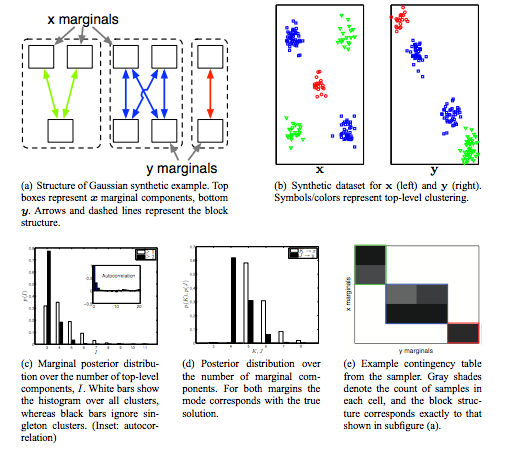
\includegraphics[width=0.9\linewidth]{multi_synth}
\end{frame}

\begin{frame}
	\frametitle{Interpretation}
	\begin{itemize}
		\item Interpretation is hard
		\item Ultimately we're interested in biological processes present in the data
		\item<2->For each gene \ac{GO} annotations are available
		\begin{itemize}
			\item These tell us what the gene is known to be involved in 
		\end{itemize}
		\item<3->We can compute whether or not a \ac{GO} term is \emph{enriched} in a cluster
		\item<4->Can do this at each posterior sample for all three types of cluster
		\item<5->Average the $p$-values across samples to obtain average values for each gene in the three cluster types.
		\item<6->Tells us if that gene is involved in that process according to mRNA, Protein, or both
		\item<7->As in previous example, the clustering is not our final goal!
	\end{itemize}
\end{frame}

\begin{frame}
	\frametitle{Results 1: what kind of blocks are present}
	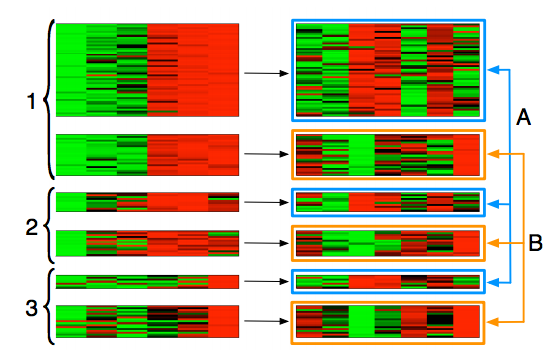
\includegraphics[width=\linewidth]{blocks}
	\begin{itemize}
		\item Highly inter-connected. Clusters on left shown by numbers, on right by letters.
	\end{itemize}
\end{frame}

\begin{frame}
	\frametitle{Results 2: what's enriched?}
	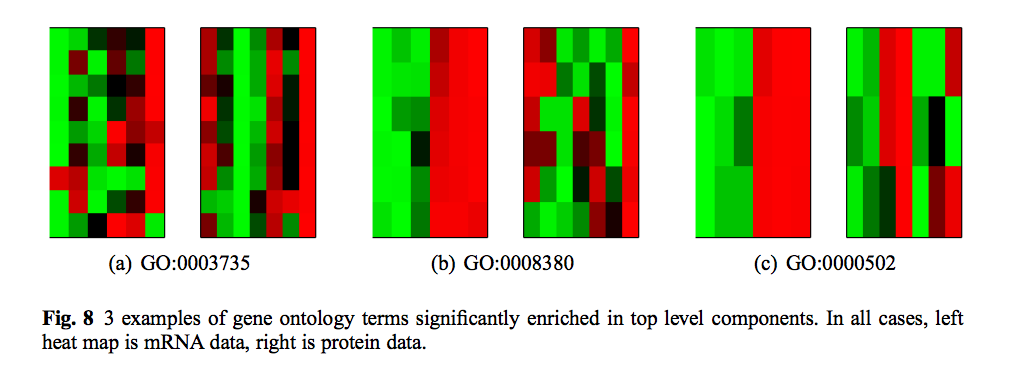
\includegraphics[width=\linewidth]{enriched_both}
	\begin{itemize}
		\item Some terms (and genes) enriched in the top components (i.e. for mRNA and protein)
	\end{itemize}
\end{frame}

\begin{frame}
	\frametitle{Results 2: what's enriched?}
	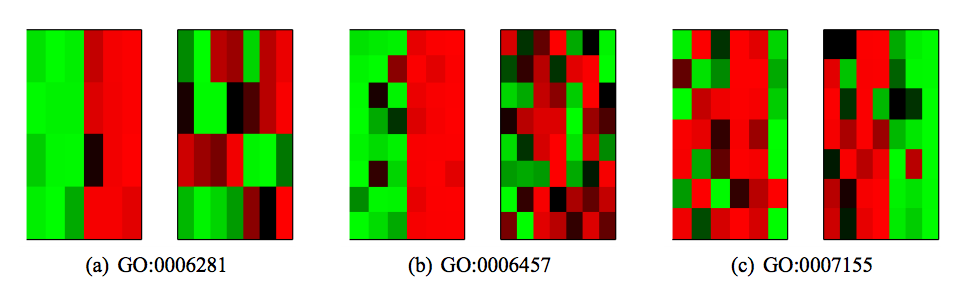
\includegraphics[width=\linewidth]{enriched_one}
	\begin{itemize}
		\item Some terms (and genes) enriched in one component and not the other (a,b: enriched in mRNC; c: enriched in protein)
	\end{itemize}
\end{frame}